\documentclass[12pt,ngerman,parskip=half]{scrartcl}

\usepackage[utf8]{inputenc}
\usepackage[T1]{fontenc}
\usepackage{booktabs}
\usepackage{babel}
\usepackage{graphicx}
\usepackage{csquotes}
\usepackage{paralist}
\usepackage{xcolor}
\usepackage{blindtext}

\usepackage{tikz}

\begin{document}

\blindtext[2]

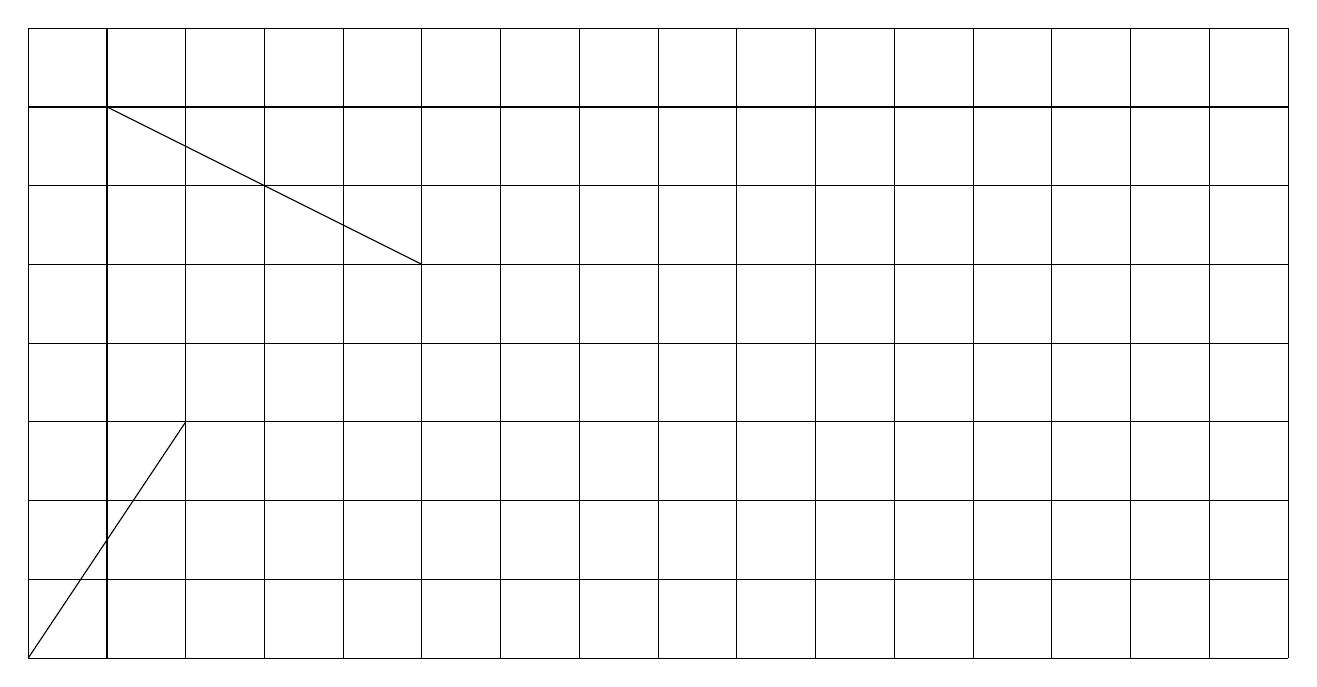
\begin{tikzpicture}
\draw (0,0) grid (16,8);
\draw (0,0) -- (2,3);
\draw (5,5) -- (1,7);
\end{tikzpicture}



\end{document}


\blindtext[1]


\begin{tikzpicture}
\draw  (0,0) grid (16,8);
\end{tikzpicture}

\blindtext[1]

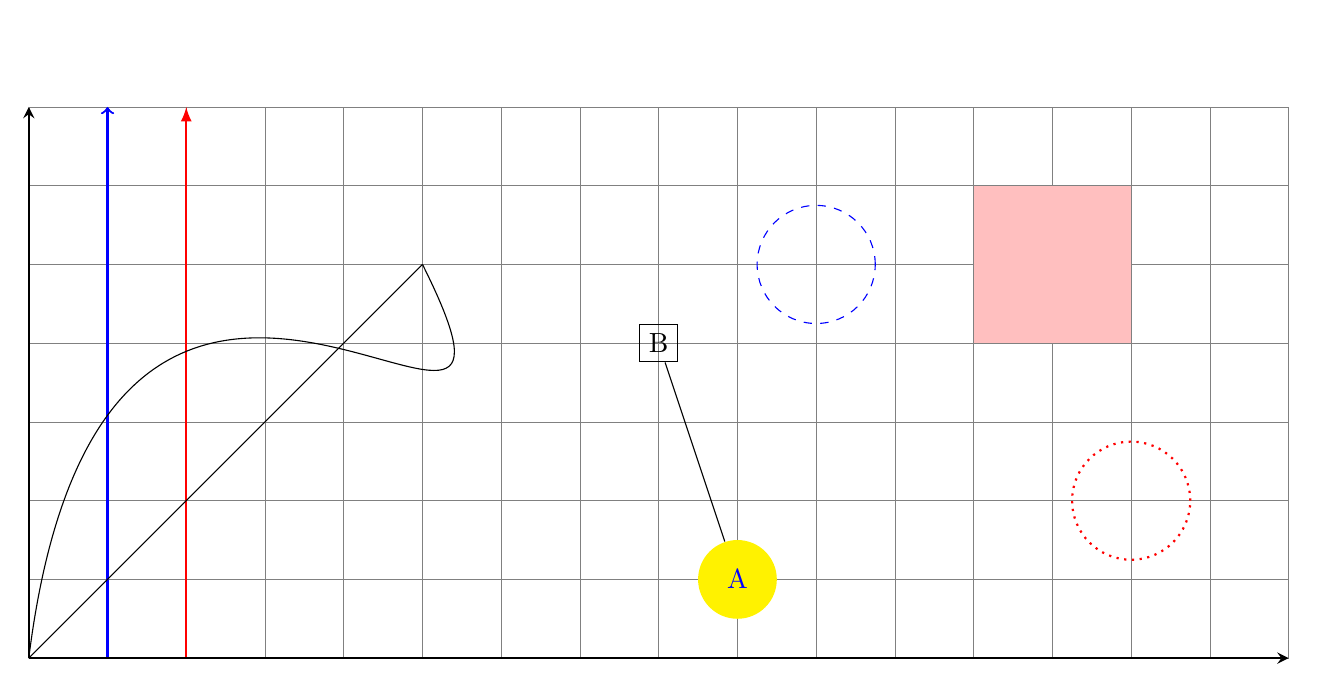
\begin{tikzpicture}[scale=1,
punkt/.style={circle, minimum size = 1cm,blue,fill=yellow},
]
\draw [gray,thick,help lines] (0,0) grid (16,7);
\draw [thick,-stealth](0,0) -- (0,7);
\draw [thick,-to,blue](1,0) -- (1,7);
\draw [red,thick,-latex](2,0) -- (2,7);
\draw [thick,-stealth](0,0) -- (16,0);

\draw (0,0) -- (5,5);
\draw (0,0) .. controls (1,8) and (7,1) .. (5,5);

\fill[red!25!white] (12,4) rectangle (14,6);

\draw[red,thick,dotted] (14,2) circle (0.75cm);

\draw[blue,dashed,thin] (10,5) circle (0.75cm);

\node[punkt] (A) at (9,1){A};
\node[draw] (B) at (8,4){B};
\draw (A) -- (B);


\end{tikzpicture}
